% $Id$
%\documentclass[handout]{beamer}
\documentclass{beamer}
\usepackage[utf8]{inputenc}
\usepackage[T1]{fontenc}
\usepackage[swedish,english]{babel}
\usepackage{url}
\usepackage{graphicx}
\usepackage{color}
\usepackage{subfig}
\usepackage{csquotes}
\usepackage{acro}
\usepackage[natbib,style=alphabetic,maxbibnames=99]{biblatex}
\addbibresource{msbintro.bib}
\DeclareAcronym{isms}
{
  short = ISMS,
  long = Information Security Management Systems,
}

\setbeamertemplate{bibliography item}[text]

\mode<presentation>{%
  \usetheme{Frankfurt}
  \setbeamercovered{transparent}
  \usecolortheme{seagull}
}
\setbeamertemplate{footline}{\insertframenumber}

\title[Intro MSB]{%
  Introduction to\\
  Swedish Civil Contingencies Agency (MSB) methodological support for introducing \acp{isms}.
}
\author{Carina Bengtsson, Daniel Bosk and Lennart Franked\footnote{%
  Detta verk är tillgängliggjort under licensen Creative Commons 
  Erkännande-DelaLika 2.5 Sverige (CC BY-SA 2.5 SE).
	För att se en sammanfattning och kopia av licenstexten besök URL 
	\url{http://creativecommons.org/licenses/by-sa/2.5/se/}.
}}
\institute[MIUN IST]{%
  Department of Informationsystem and Technologies (IST),\\
  Mid Sweden University, Sundsvall.
	
  %Avdelningen för informations- och kommunikationssytem (IKS),\\
  %Mittuniversitetet, Sundsvall.
}
\date{\today}

%\pgfdeclareimage[height=0.65cm]{university-logo}{MU_logotyp_int_CMYK.pdf}
%\logo{\pgfuseimage{university-logo}}

\AtBeginSection[]{%
	\begin{frame}<beamer>{Overview}
		\tableofcontents[currentsection]
	\end{frame}
}

\begin{document}

\begin{frame}
  \titlepage{}
\end{frame}

\begin{frame}{Overview}
	\tableofcontents
	% You might wish to add the option [pausesections]
\end{frame}


% Since this a solution template for a generic talk, very little can
% be said about how it should be structured. However, the talk length
% of between 15min and 45min and the theme suggest that you stick to
% the following rules:  

% - Exactly two or three sections (other than the summary).
% - At *most* three subsections per section.
% - Talk about 30s to 2min per frame. So there should be between about
%   15 and 30 frames, all told.


\section[Methodilogical support]{MSB:s methodological support}

\subsection{MSB}

\begin{frame}{MSB}
  \begin{itemize}
    \item Swedish Civil Contingencies Agency (MSB).
    \item \enquote{MSB is responsible for issues concerning civil protection,
        public safety, emergency management and civil defence, as long as no
        other authority has responsibility\cite[About MSB]{msbse}\@.
        .}
  \end{itemize}
\end{frame}

%\begin{frame}{MSB:s organisation}
%  \begin{figure}
%    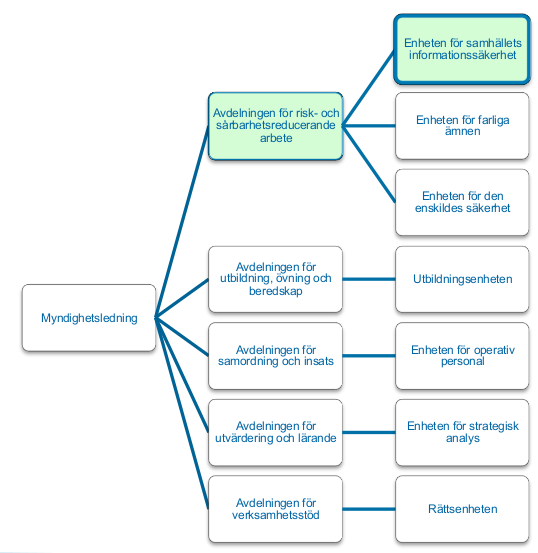
\includegraphics[height=0.7\textheight]{msb-organisation.png}
%    \caption{MSB:s organisation.}
%  \end{figure}
%\end{frame}

\begin{frame}{Why do we as a society need this?}
  \begin{itemize}
    \item Information is central in today's society.
    \item Accommodates the need for both the individual and the society.
    \item Necessary to avoid disturbances in our information systems.
  \end{itemize}
\end{frame}

\begin{frame}[allowframebreaks]{Tieto-breakdown}
  \citet{Lindkvist2012tdf} gives the following summary:
  \begin{description}
    \item[Friday afternoon] Tieto notices a disruption in their IT-systems.
      350 pharmacies lost contact with their IT-systems.
      Many larger organisations are also affected, amongst other a larger
      logistical company.

    \item[Sunday afternoon] Tieto is reporting hardware malfunction, and start
     the necessary steps to fix the malfunction.

    \item[Monday morning] The logistical company are unable to handle its
      operation, and cannot reach its employees.
      The vehicle inspection agency are unable to access their IT-system. Since
      they were handling over 20\, 000 vehicle inspections a day, it might
      result to a driving ban for some vehicles, since they cannot report
      approved inspections.
      Nacka municipality, have to resort to Facebook and Twitter for
      communicating within the municipality.

    \item[Monday afternoon] Social office in Nacka and Sollentuna are unable to
      pay child support.
      Stockholm City absence reporting system for the schools are down.

    \item[Wednesday lunch] All the pharmacies have gotten access to their
      IT-systems again.

    \item[11 days] The logistical company can start using their IT-system.
      The organisation where still recovering from the disruption, two months
      after.
  \end{description}
\end{frame}

\subsection{Methodological support}

\begin{frame}{Informationssäkerhet.se}
  \begin{itemize}
    \item MSB ran a project called SVISA\@: 'Stöd för Verksamheters 
      InformationsSäkerhetsArbete'.

    \item Resulted in \url{informationssäkerhet.se}.

    \item Is meant to give practical advice for systematically incorporate
      information security into an organisation.
  \end{itemize}
\end{frame}

\begin{frame}{Methodological support}
  \begin{itemize}
    \item Support for how to conduct work within information security in an
      organisation.

    \item Explains how to build an information security management system.

    \item Should be seen as a \enquote{smorgasbord}:
      \begin{itemize}
        \item Pick the parts that are related to the organisation.
        \item Apply them in an order that is suitable.
      \end{itemize}

    \item Information security is a complex field:
      \begin{itemize}
        \item It is required that it is integrated in the \emph{entire}
          organisation: From the top management to the lowest operative level.
      \end{itemize}

  \end{itemize}
\end{frame}

\begin{frame}{Methodological overview}
  \begin{figure}
    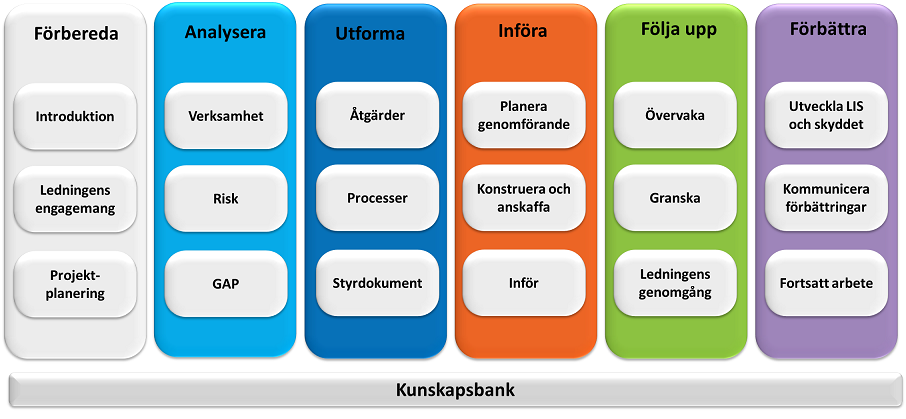
\includegraphics[width=\textwidth]{metodstod-overview.png}
    \caption{Overview over the methodological support.}
  \end{figure}
\end{frame}

\section{Prepare}

\subsection{Introduction}

\begin{frame}{What is information security?}
  \begin{itemize}
    \item Occurs together with other processes and organisations.

    \item Information security in an organisation does not have a value by
      itself. It needs to be integrated into the organisation to be effective.

  \end{itemize}
\end{frame}

\begin{frame}{What is information security?}
  \begin{itemize}
    \item Ability to preserve the requirements and expectations that exist on
      information in an organisation.

    \item Amongst other to protect towards disruptions, such as what happened to
      Tieto.

  \end{itemize}
\end{frame}

\begin{frame}{Demands and expectations on information}
  \begin{description}
    \item[Confidentiality] The information should only be accessible to an
      authorized entity.

    \item[Availability] The information must be accessible when it is needed.

    \item[Integrity] The information is exact and complete.

  \end{description}
\end{frame}

\begin{frame}{Demands and expectations on information}
  \begin{description}
    \item[Traceability] Who have taken part of, or changed the information?
    \item[Non Repudiation] It should not be possible to deny an act.
    \item[Authentication] Establish an entities identity.
    \item[Authorization] To give an authenticated entity certain permissions.
  \end{description}
  These will be covered later in the course.
\end{frame}

\begin{frame}{What is information security?}
  \begin{figure}
    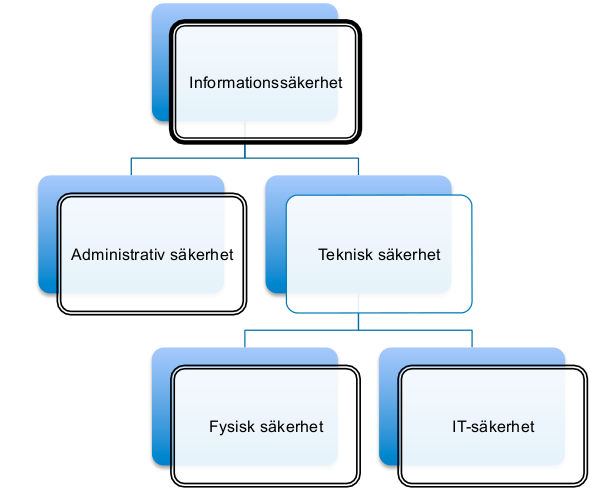
\includegraphics[height=0.7\textheight]{infosak-struktur.png}
    \caption{Structure of information security.}
  \end{figure}
\end{frame}

\begin{frame}{Structure}
  \begin{figure}
    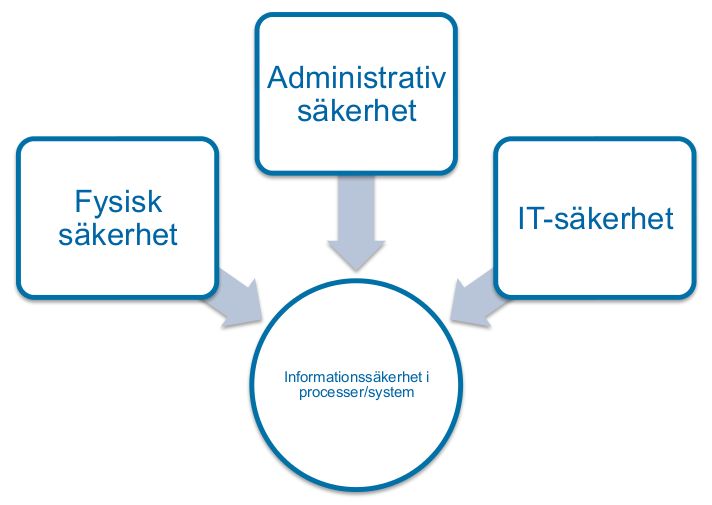
\includegraphics[height=0.7\textheight]{infosak-process.png}
    \caption{To work with information security}
  \end{figure}
\end{frame}

\begin{frame}{The security isn't stronger than the weakest link}
  \begin{itemize}
    \item Strong password, written down on a post-it next to where it should be
      used.
    \item High grade lock on a regular glass door.
    \item The conditions must be there, in order to be able to work safely.
  \end{itemize}
\end{frame}

\begin{frame}{Why protect the information?}{Non-mandatory}
  \enquote{Good for business}
  \begin{description}
    \item[Reputation:] Who will let a company handle their information, if the
      company is known for treating their data carelessly.

    \item[Financial:] Strong reputation is better for the economy, and the cost
      of dealing with security incidents will be less.

    \item[Internal efficiency:] No loss of information or disruptions in the
      work.

    \item[Quality:] This will hopefully lead to a increase in work quality.

  \end{description}
\end{frame}

\begin{frame}{Why protect the information?}{Mandatory}
  \begin{description}
    \item[Personal Data Act 1998:204] adds restrictions on how an organisation manages
      personal data.

    \item[Public Access to Information and Secrecy Act 2009:40] Says that certain
      information \emph{must} be available for the public, while other information
      should \emph{not} be.

    \item[The Archives Act 1990:782] says that the government needs to archive
      all public documents.

    \item[MSBFS 2016:1] applies to governmental agency and their
      work with information security.

  \end{description}
\end{frame}

\begin{frame}{MSBFS 2016:1}
  \begin{itemize}
    \item Due to increased electronic information exchange in the society, there
      is now demands put on how governmental agency work with information
      security.

    \item The code of statutes came into effect 1th of February 2010.

  \end{itemize}
\end{frame}

\begin{frame}{MSBFS 2016:1}
  1 §  Denna författning innehåller föreskrifter som ansluter till
  bestämmelserna om statliga myndigheters informationssäkerhet i 19§
  förordningen (2015:1052) om krisberedskap och bevakningsansvariga
  myndigheters åtgärder vid höjd beredskap. 

\end{frame}

\begin{frame}{MSBFS 2016:1}
  5 §  Varje myndighet ska bedriva ett systematiskt och riskbaserat
  informationssäkerhetsarbete med stöd av ett ledningssystem för
  informationssäkerhet. I detta arbete ska standarderna ISO/IEC 27001:2014 och
  ISO/IEC 27002:2014 beaktas. Tillräckliga resurser ska tilldelas för
  informationssäkerhetsarbetet samt löpande och regelbunden information lämnas
  till myndighetsledningen.
  
  Detta innebär bland annat att en myndighet måste: 
  \begin{enumerate}
    \item upprätta en informationssäkerhetspolicy och andra styrande dokument 
      som behövs för myndighetens informationssäkerhet,
    \item utse en eller flera personer som leder och samordnar arbetet med 
      informationssäkerhet,
    \item klassificera sin information med utgångspunkt i krav på 
      konfidentialitet, riktighet och tillgänglighet,
    \item utifrån risk- och sårbarhetsanalyser och inträffade incidenter 
      avgöra hur risker ska hanteras, samt besl uta om åtgärder för 
      myndighetens informationssäkerhet,
    \item dokumentera granskningar och säkerhetsåtgärder av större betydelse 
      som har vidtagits.
    \item 
  \end{enumerate}
\end{frame}

\begin{frame}{MSBFS 2016:1}
  10 § Myndigheten ska ha rutiner för att identifiera, rapportera, bedöma,
  hantera och dokumentera incidenter som kan påverka säkerheten i den
  informationshantering som myndigheten ansvarar för eller i tjänster som
  myndigheten tillhandahåller åt en annan organisation. Myndigheten ska ha
  rutiner för att lära av sådana inträffade incidenter och utförda åtgärder. 
\end{frame}

\begin{frame}{ISO 27000}
  \begin{itemize}
    \item This is not just for governmental agencies.

    \item Any organisation can certify themselves for ISO27000

    \item MSB:s methodological support is adapted to the international
      standards.

  \end{itemize}
\end{frame}

\begin{frame}{Management System}
  \begin{itemize}
    \item Everyone have a \enquote{system} to manage an organisation.
  \end{itemize}
      A formalized system that is used to make the work more efficient in
      regards to set goals. It should include routines and delegation of
      responsibilities for how the organisation should be managed. It must exist
      clear goals and guidelines for how they should be achieved.
  \begin{itemize}
    \item Covers amongst other, organisational structures, governance documents
      etc.
  \end{itemize}
\end{frame}

\begin{frame}{Information Security Management System (ISMS)}
  \begin{itemize}
    \item Should be integrated with the other management systems!
    \item Refers to how to regulate the work with information security.
    \item Also how to regulate work routines, methods \dots
    \item Governance documents have an important role to play in \acp{isms}\@.
  \end{itemize}
\end{frame}

\begin{frame}{Apply \acp{isms}}
  Not only establish, but also
  \begin{itemize}
    \item implement,
    \item pursue,
    \item monitor,
    \item audit,
    \item maintain and improve
  \end{itemize}
\end{frame}

\begin{frame}{Governance documents}
  \begin{itemize}
    \item Plan of action, policies, guidelines, \dots

    \item Policy: What do we want to achieve?
      One extensive, or multiple smaller ones.

    \item The governance documents should be integrated into the organisations
      current structure.

  \end{itemize}
\end{frame}

\begin{frame}{Information security in different levels}
  \begin{figure}
    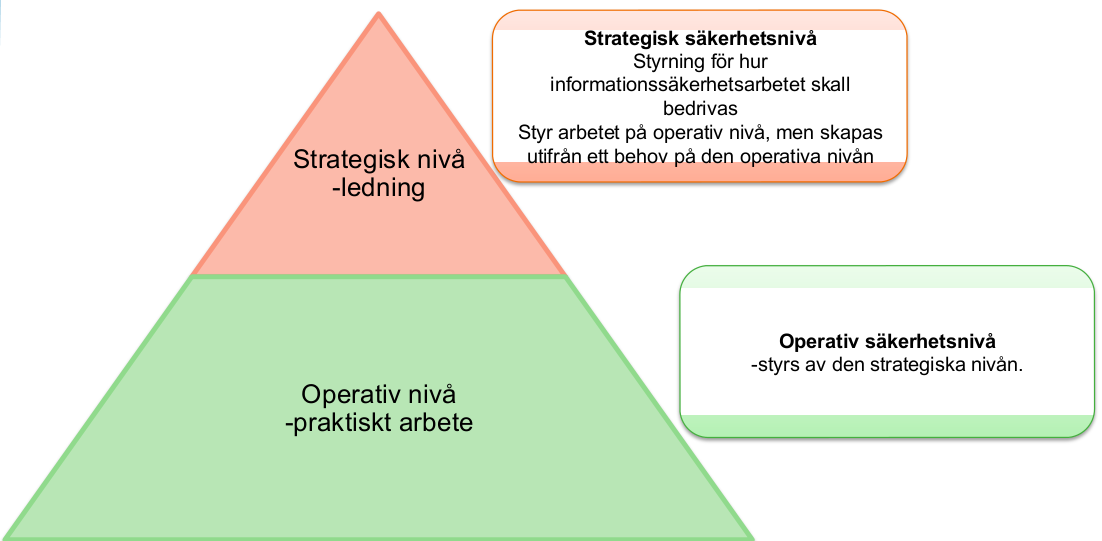
\includegraphics[width=\textwidth]{infosak-levels.png}
    \caption{Different levels where information security can be conducted.}
  \end{figure}
\end{frame}

\begin{frame}{Purpose with \acp{isms}}
  \begin{figure}
    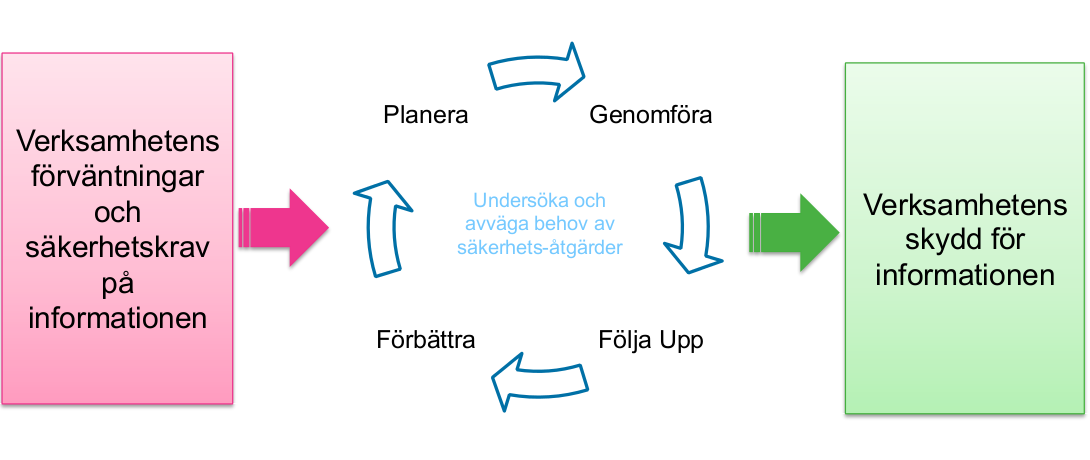
\includegraphics[width=\textwidth]{infosak-pdca.png}
    \caption{To convert requirements to an active protection.}
  \end{figure}
\end{frame}

\begin{frame}{ISO 27001}
  \begin{itemize}
    \item MSB's methodological support, describes how to build an \acp{isms},
      based on ISO 27001.

    \item ISO 27001 is a continuous process that strives towards constant
      improvements on how to work and use different security solutions in
      regards to information security.

    \item It is important to adapt this after the organisation, but this does
      not mean that parts can be skipped.

  \end{itemize}
\end{frame}

\begin{frame}{PDCA}
  \begin{description}
    \item[Plan] Plan, analyze and design.
    \item[Do] Establish.
    \item[Check] Follow up.
    \item[Act] Improve.
  \end{description}
  Then start over again.
\end{frame}

\begin{frame}{ISO 27002 -- What should be done?}
  \begin{itemize}
    \item Security Policy.
    \item Organising the information security.
    \item Managing assets.
    \item Human resource and security.
    \item Physical and environmental security.
    \item Control communication and management.
    \item Access control.
    \item Acquisition, development and maintenance of information systems.
    \item Managing information security incidents.
    \item Continuity planning for the organisations.
    \item Compliance.
  \end{itemize}
\end{frame}

\begin{frame}{ISO 27002 -- What should be done?}
  All of this is covered in different chapters in ISO 27002. We will cover parts
  of this during the next lecture.
\end{frame}

\subsection{Committed Management}

\begin{frame}{Committed management}
  \begin{itemize}
    \item How to succeed?
      Support is needed from the top management.

    \item Since the work with information security should cover the entire
      organisation, it is vital that the top management is fully committed.

    \item Those that have been appointed to work with information security,
      needs to have the mandate to be able to do their work.

  \end{itemize}
\end{frame}

\begin{frame}{Create commitment}
  \begin{itemize}
    \item The top management have the overall responsibility for the
      organisation -- This involves information security and security incidents.
      
    \item Important to make the management understand the importance of
      information security.

  \end{itemize}
\end{frame}

\begin{frame}{Motivation}
  \begin{itemize}
    \item What positive effects might come with strong information security?

    \item What is the price of \emph{not} protecting the information?
      \begin{itemize}
        \item Leaked company secrets.
        \item Inaccessible infrastructure.
      \end{itemize}

    \item Show incidents.

    \item Laws and other regulations?

  \end{itemize}
\end{frame}

\subsection{Project planning}

\begin{frame}{Project planning}
  \begin{itemize}
    \item MSB recommends that an \acp{isms} should start in project form and
      then go over to become a process.
  \end{itemize}
  \begin{figure}
    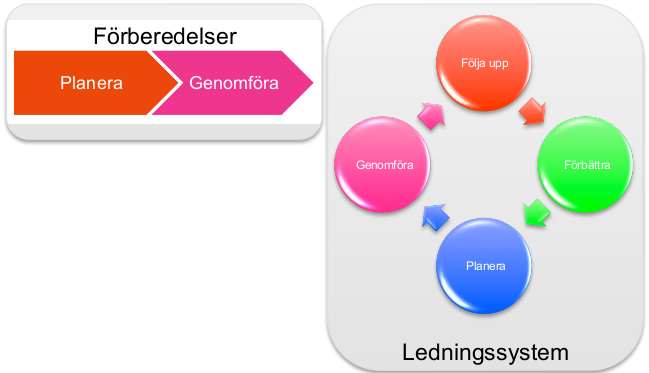
\includegraphics[height=0.5\textheight]{lis.png}
    \caption{Establish and implement an \acp{isms}.}
  \end{figure}
\end{frame}

\begin{frame}{Project plan}
  \begin{itemize}
    \item The foundation of the project.
    \item Defines the extent of the \acp{isms}\@.
    \item An agreement that is good for both the project leader and the
      management.
    \item Can contain:
      \begin{itemize}
        \item Background and need,
        \item purpose,
        \item goal,
        \item extent och demarcation,
        \item connections and contact surfaces,
        \item time plan, and
        \item budget.
      \end{itemize}
  \end{itemize}
\end{frame}

\begin{frame}{Organising the project}
  \begin{itemize}
    \item Important with wide knowledge: to represent the entire organisation.
    \item Important with the correct qualifications: leading projects, and
      information security.
    \item Important with mandates!
    \item The organisation should be active and engaged, so that the competence
      is not gone once the project is over.
  \end{itemize}
\end{frame}

\begin{frame}{A short checklist}
  \begin{itemize}
    \item Have the management made a decision to implement \acp{isms}?
    \item Have the management appointed someone to coordinate the organisations
      work with information security?
    \item Have the management ensured that there is a strategy to communicate
      the work with \acp{isms} internally?
    \item Have the management made a decision regarding the budget and
      resources?
  \end{itemize}
\end{frame}

\section{Analyze}

\subsection{Organisational analysis}

\begin{frame}{What should be protected?}
  \begin{itemize}
    \item What information assets do we have, and are they worth protecting?
    \item What does it mean to protect them?
  \end{itemize}
\end{frame}

\begin{frame}{Organisational analysis}
  \begin{itemize}
    \item The purpose of the organisational analysis is to identify the
      informational assets available, and 

    \item find how much they are worth protecting.

    \item Should lead to a structured list over
      \begin{itemize}
        \item what informational assets there are,
        \item what requirements and expectations they have, and 
        \item the worth of each asset.
      \end{itemize}

  \end{itemize}
\end{frame}

\begin{frame}{Example of informational assets}
  \begin{itemize}
    \item Employees: qualifications and experiences.
    \item Data: databases, agreement, documentation, samples, routines.
    \item Access to software: application software, system software, 
      development software.
    \item Services: data- and communication systems, supply systems.
    \item Immaterial: reputation, profile.
    \item Physical: computer equipment, movable media.
  \end{itemize}
\end{frame}

\begin{frame}{Dividing informational assets}
  \begin{description}
    \item[Primary] Refers to the main information, such as blue prints, logs or
      contracts.

    \item[Secondary] Refers to resources that are required to access the primary
      informational assets.

  \end{description}
  What will happen if you do not have your program that is required to read the
  closed proprietary format that the information is stored with?

\end{frame}

\begin{frame}{Finding the informational assets}
  \begin{itemize}
    \item Previous process mappings?
    \item Department wise?
    \item IT-system?
    \item Project?
    \item Processes?
    \item By function?
  \end{itemize}
\end{frame}

\begin{frame}{Requirements on the informational assets}
  \begin{itemize}
    \item In order to be able to classify, the requirements needs to be known.

    \item Necessary to be able to objectively measure the need for protection.
      \begin{itemize}
        \item My information is the most important!
      \end{itemize}

    \item What information is necessary for the organisation?

  \end{itemize}
\end{frame}

\begin{frame}{Legal requirements}
  Agreement, laws and regulations.
  \begin{itemize}
    \item Personal Data Act,
    \item The Archives Act,
    \item Public Access to Information and Secrecy Act
    \item MSBFS 2016:1,
    \item Security Act.
  \end{itemize}
\end{frame}

\begin{frame}{Internal requirements}
  Requirements that the organisation have to reach its goals.
  For example:
  \begin{itemize}
    \item Vision,
    \item Business concept,
    \item policies,
    \item values.
  \end{itemize}
\end{frame}

\begin{frame}{Classifying information}
  \begin{itemize}
    \item Method to evaluate how much an informational asset is worth
      protecting.

    \item To be able to create a suitable protection.

    \item Evaluate each asset based on:
      \begin{itemize}
        \item Availability,
        \item Integrity,
        \item Confidentiality.
      \end{itemize}

    \item Each perspective have a number of security levels.

  \end{itemize}
\end{frame}

\begin{frame}{MSB:s suggestion on a classification model}
  \begin{figure}
    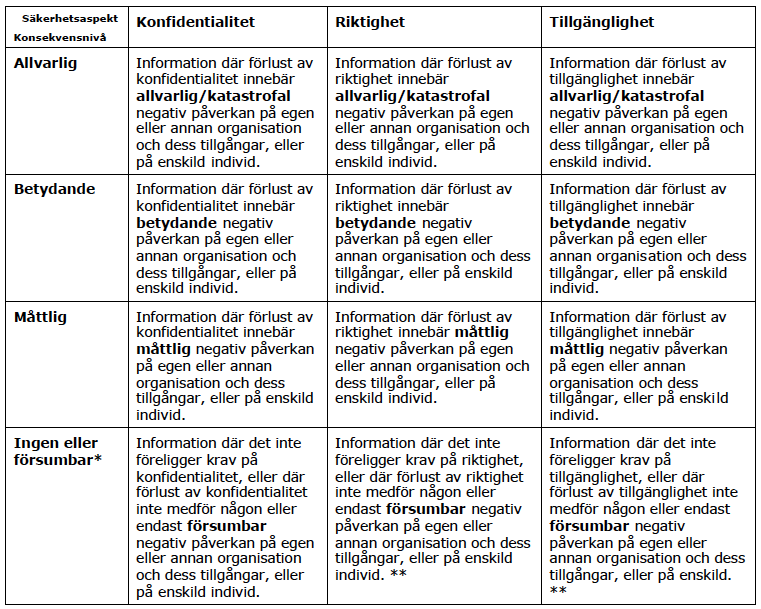
\includegraphics[height=0.7\textheight]{msb-klassificering.png}
    \caption{MSB:s suggestion on a classification model.}
  \end{figure}
\end{frame}

\begin{frame}{Classifying information}
  \begin{itemize}
    \item All assets are classified using all the identified requirements based
      on all the different perspectives.
    \item The information owner should be the one classifying the information.
    \item It is good to adapt the model based on the organisation.
  \end{itemize}
\end{frame}

\begin{frame}{University's adaptation of a classification model.}
  \begin{figure}
    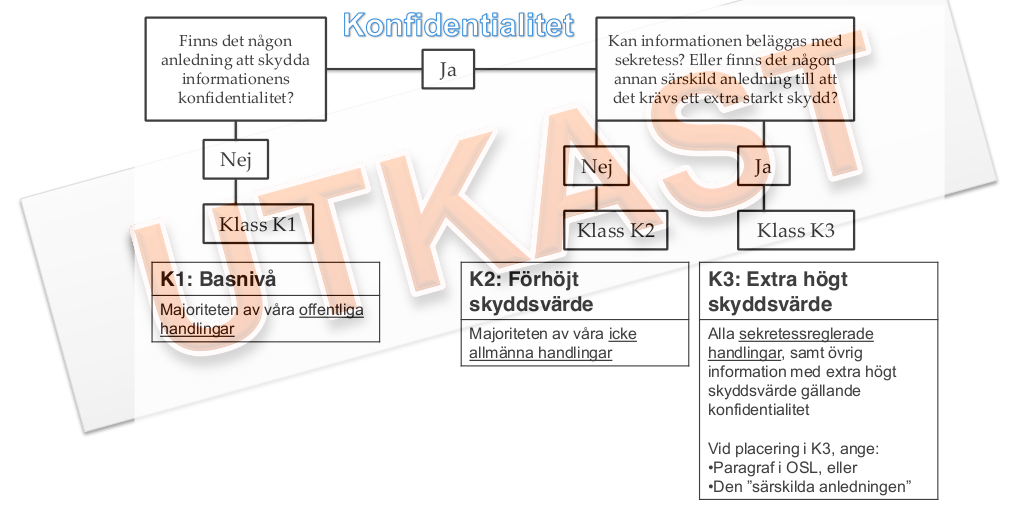
\includegraphics[width=\textwidth]{miun-klassificering.png}
    \caption{University's adaptation of a classification model from the
      confidentiality perspective.}
  \end{figure}
\end{frame}

\begin{frame}{University's adaptation of a classification model}
  \begin{figure}
    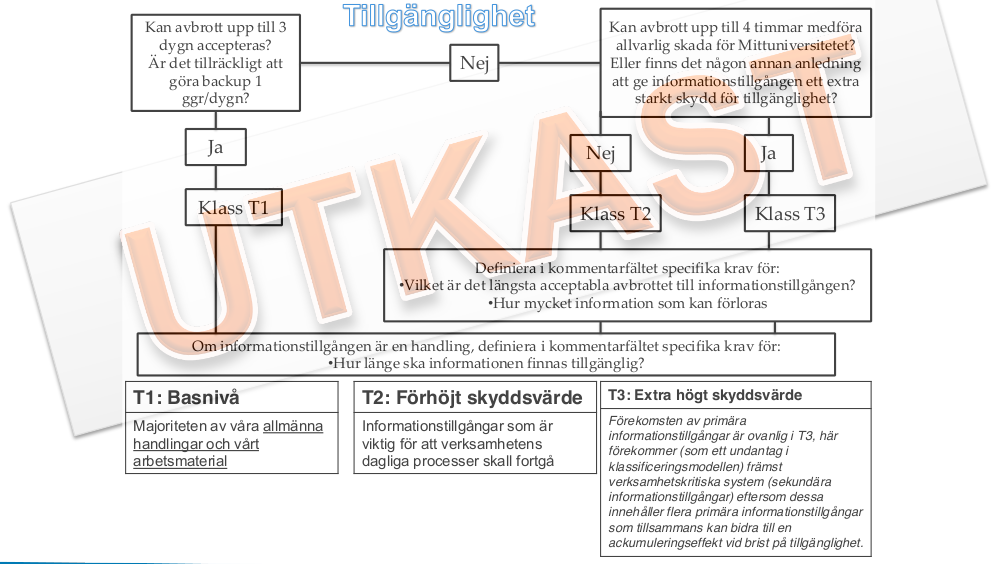
\includegraphics[width=\textwidth]{miun-tillganglighet.png}
    \caption{University's adaptation of a classification model from the
      availability perspective.}
  \end{figure}
\end{frame}

\begin{frame}{University's adaptation of a classification model}
  \begin{figure}
    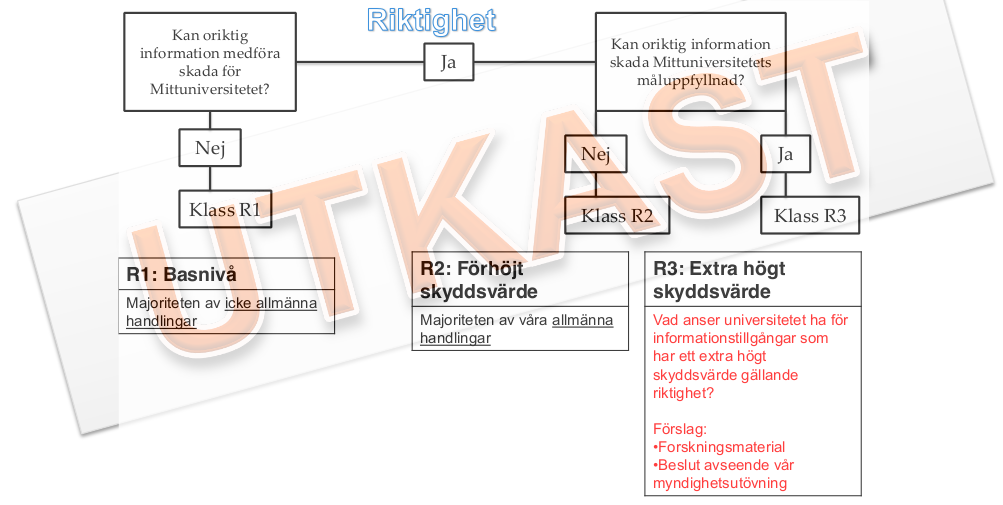
\includegraphics[width=\textwidth]{miun-riktighet.png}
    \caption{University's adaptation of a classification model from the
      integrity perspective.}
  \end{figure}
\end{frame}

\begin{frame}{Example of the result from the university}
  \begin{figure}
    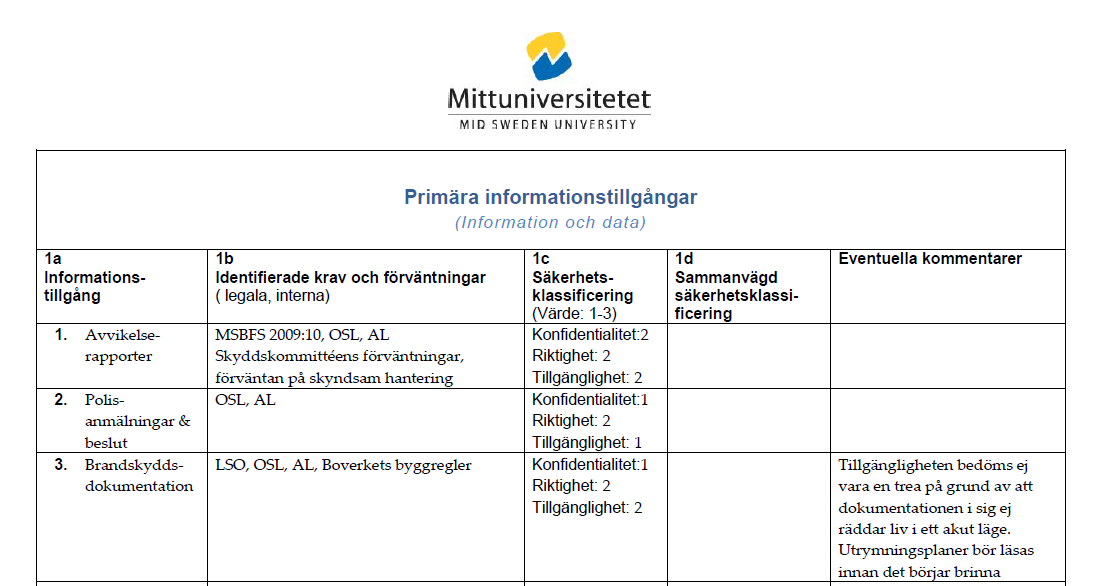
\includegraphics[width=\textwidth]{miun-klassresultat.png}
    \caption{Part of the result from the university.}
  \end{figure}
\end{frame}

\subsection{Risk analysis}

\begin{frame}{Risk analysis}
  Necessary for demarcation:
  \begin{itemize}
    \item What informational assets should we do a risk analysis on?
    \item What informational assets are not critical enough for a risk analysis?
  \end{itemize}
\end{frame}

\begin{frame}{Risk analysis}
  \begin{itemize}
    \item Used to adapt the protection based on the assets of the organisation.
    \item Generate a list over
      \begin{itemize}
        \item existing threats,
        \item consequences of the threats, and
        \item suggestions for risk management.
      \end{itemize}
  \end{itemize}
\end{frame}

\begin{frame}{Identify threats}
  \begin{itemize}
    \item Use brain storming to find potential threats.
    \item Include all the suggestions!
    \item Be specific: Intensional or unintentional information leakage.
    \item Example:
      \begin{itemize}
        \item An employee intentionally sabotages a system.
        \item An employee accidentally trips on a network cable.
        \item Software bug.
        \item Fire, flooding.
      \end{itemize}
  \end{itemize}
\end{frame}

\begin{frame}{Risk matrix}
  \begin{figure}
    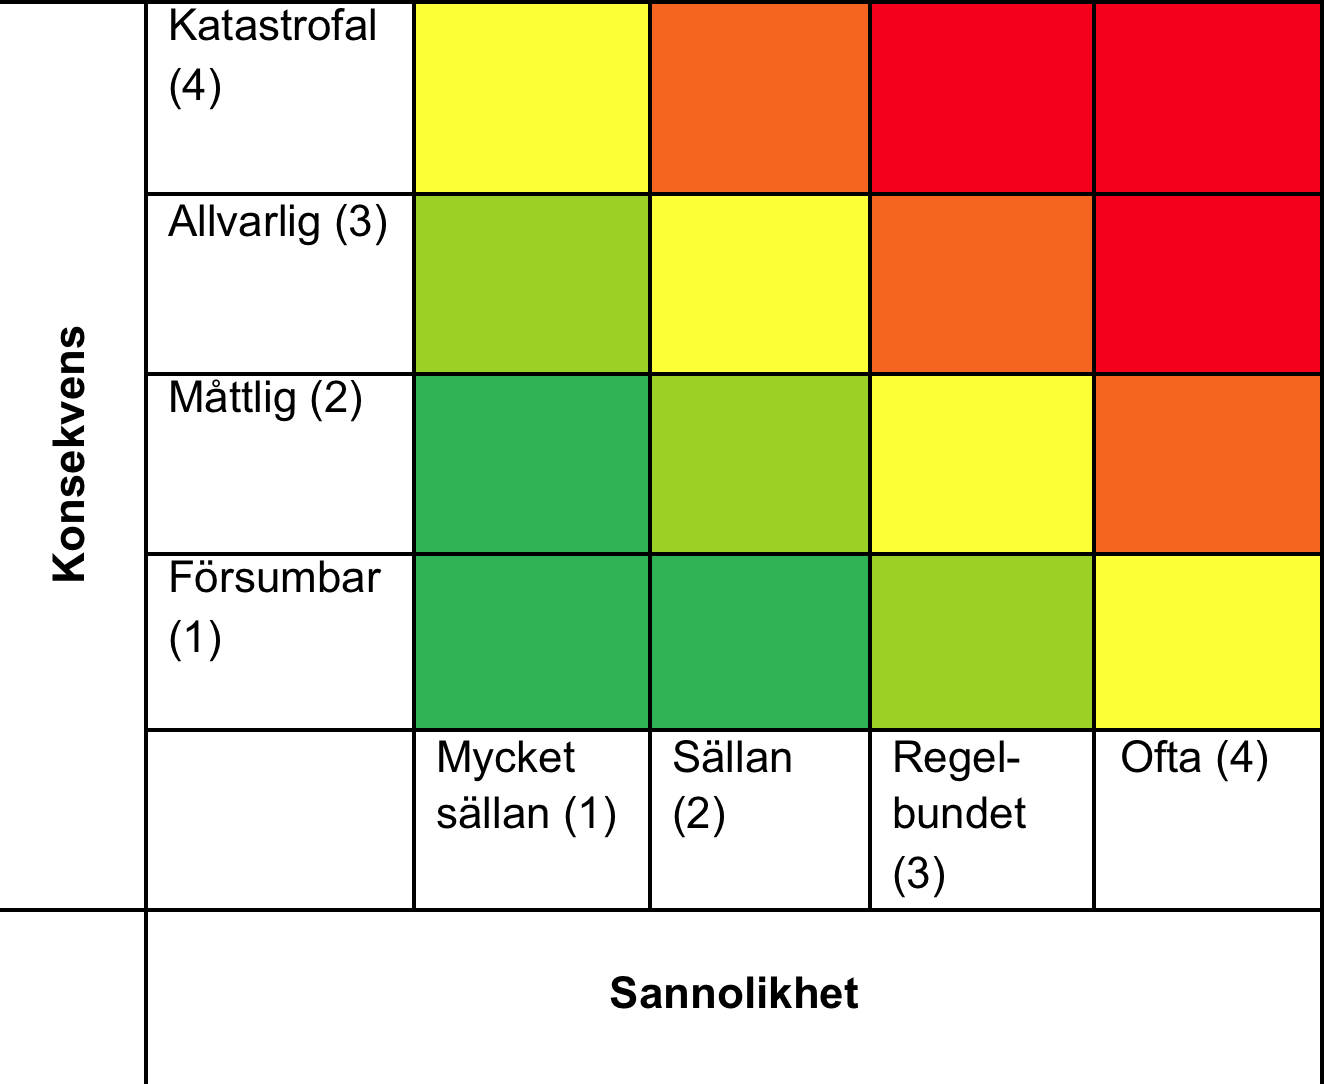
\includegraphics[height=0.7\textheight]{riskmatris.png}
    \caption{A risk matrix.}
  \end{figure}
\end{frame}

\begin{frame}{Risk matrix}
  \begin{itemize}
    \item Assess the probability and the consequence of each individual threat,
      and place them in the matrix.
    \item The focus on consequences should be consequences for the organisation.
    \item Gives a visual result, easily understandable and gives a good overview
      of how to prioritize security measures.
  \end{itemize}
\end{frame}

\begin{frame}{Risk matrix}{Consequences}
  \begin{itemize}
    \item How severe is the consequence for the organisation of the threat
      happens?
    \item Clarify who will be a affected: Organisation through a side effect of
      consequences in the society? 
    \item Makes it easier to give examples for the different consequence levels.
      For example: loss of reputation, higher cost, \dots.
  \end{itemize}
  \begin{center}
    Severe -- Considerable -- Moderate -- Negligible
  \end{center}
\end{frame}

\begin{frame}{Risk matrix}{Probability}
  \begin{itemize}
    \item What is the probability that the threat occur?
    \item Makes it easier to give examples for the different levels: Years,
      weeks, days?
  \end{itemize}
  \begin{center}
    Very rarely -- Rare -- Regularly -- Often
  \end{center}
\end{frame}

\begin{frame}{Risk management}
  \begin{itemize}
    \item Decide whether the identified threats should be rectified or be
      accepted:
      \begin{itemize}
        \item Accept,
        \item eliminate,
        \item transfer,
        \item rectify.
      \end{itemize}
    \item What measures should be taken?
  \end{itemize}
\end{frame}

\begin{frame}{Possible measures}
  \begin{itemize}
    \item Administrative security:
      \begin{itemize}
        \item Governance documents,
        \item Educational measures.
      \end{itemize}
    \item Physical security:
      \begin{itemize}
        \item Access control,
        \item Locked cabinets.
      \end{itemize}
    \item IT-security:
      \begin{itemize}
        \item Firewalls,
        \item Encryption,
        \item The course will cover more possible measures.
      \end{itemize}
  \end{itemize}
\end{frame}

\begin{frame}{University example}
  Classified research material with large commercial interest: K3, R2 and T2.
  \begin{figure}
    \hfill
    \subfloat[Threat assessment]{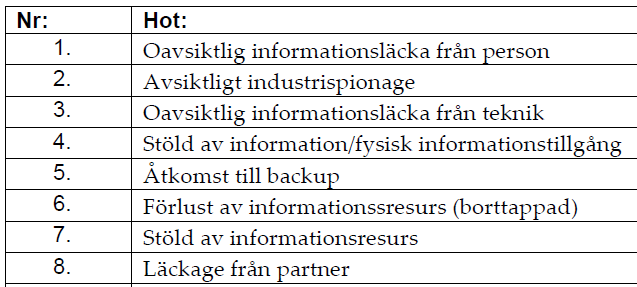
\includegraphics[width=0.4\textwidth]{miun-hot.png}}
    \hfill
    \subfloat[Risks]{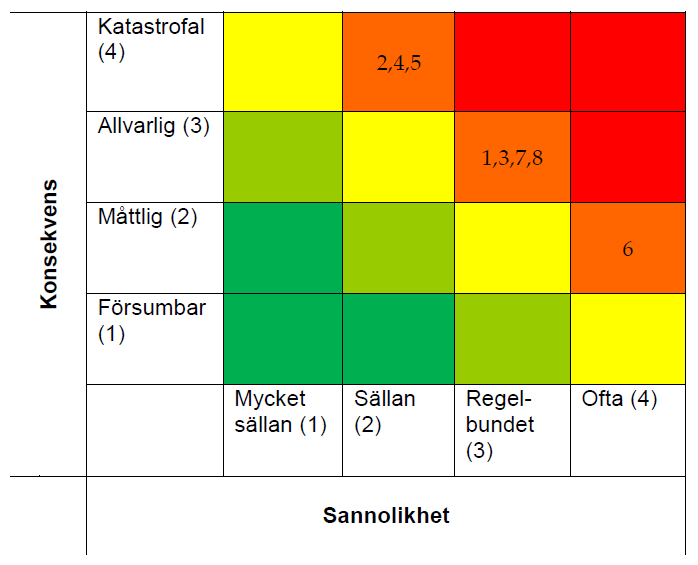
\includegraphics[width=0.4\textwidth]{miun-riskmatris.png}}
    \hfill
    \caption{Threat assessment and assessed risk.}
  \end{figure}
\end{frame}

\begin{frame}{University example}
  \begin{figure}
    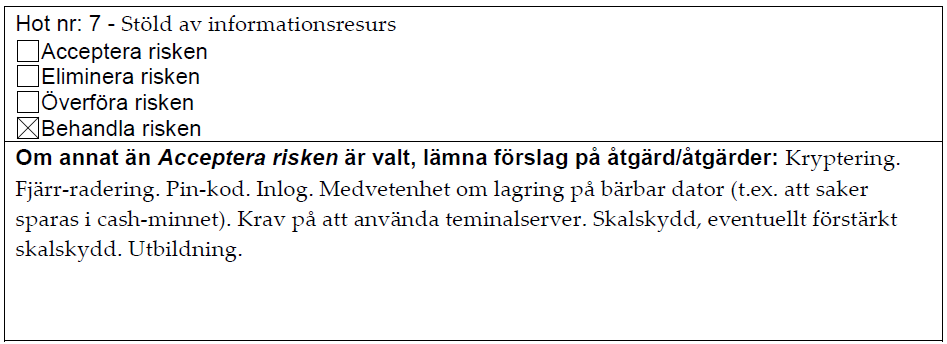
\includegraphics[width=\textwidth]{miun-atgard.png}
    \caption{Measures to address the threat.}
  \end{figure}
\end{frame}

\begin{frame}{Finally---when should the risk analysis be done?}
  \begin{itemize}
    \item Yearly.
    \item With organisational change.
    \item When planning a new organisation.
  \end{itemize}
\end{frame}


\section[Assignments]{Examination}

\begin{frame}{Examination}
  \begin{itemize}
    \item M1 Information Security Management System.
    \item M2 Organisational and risk analysis.
    \item S3 Organisational and risk analyses.
  \end{itemize}
\end{frame}


%%%%%%%%%%%%%%%%%%%%%%

\begin{frame}[allowframebreaks]{References}
  \small
  \printbibliography{}
\end{frame}

\end{document}

